%%%%%%%%%%%%%%%%%%%%%%%%%%%%%%%%%%%%%%%%%%%%%%%%%%%%%%%%%%%%%%%%%%%%%%%%%%%%%%%%
%2345678901234567890123456789012345678901234567890123456789012345678901234567890
%        1         2         3         4         5         6         7         8

\documentclass[letterpaper, 10 pt, conference]{ieeeconf}  % Comment this line out
                                                          % if you need a4paper
%\documentclass[a4paper, 10pt, conference]{ieeeconf}      % Use this line for a4
                                                          % paper

\IEEEoverridecommandlockouts                              % This command is only
                                                          % needed if you want to
                                                          % use the \thanks command
\overrideIEEEmargins
% See the \addtolength command later in the file to balance the column lengths
% on the last page of the document

\usepackage{graphicx,graphics}
\usepackage{amssymb,amsmath}
\usepackage{amsfonts}
% \usepackage{calrsfs} % for calligraphic font in math mode
\usepackage{subfigure}
\usepackage{url}
\usepackage{color}
\usepackage{algorithm}
\usepackage{algorithmicx}
\usepackage{algpseudocode}
\usepackage[table,xcdraw]{xcolor}
\usepackage{xargs}[2008/03/08]
\newcommand{\mfcomment}[1]{{\color{blue}[MF: #1]}}
\newcommand{\stcomment}[1]{{\color{blue}[ST: #1]}}


\title{\LARGE \bf
Deep Turtle Control
}

\author{Michael Farrell, Skyler Tolman}
\begin{document}

\maketitle
\thispagestyle{empty}
\pagestyle{empty}

\begin{abstract}
    abstract here
\end{abstract}

%%%%%%%%%%%%%%%%%%%%%%%%%%%%%%%%%%%%%%%%%%%%%%%%%%%%%%%%%%%%%%%%%%%%%%%
% !TEX root=../main.tex
\section{Introduction}
\label{sec:intro}

% A brief introduction to the project.
% Make sure to explain why it's important/relevant/interesting.
% Briefly summarize relevant papers that you build your project on.

Over the past decade, the deep learning revolution has quickly made its way into
many applications and products. During the same time frame, the self-driving car
has rapidly become the focus of many companies ranging from start-ups to tech
giants. It is no mistake that these two movements have gained traction at the
same time. State-of-the-art approaches to the self-driving car problem depend on
a fusion on classical methods with deep
learning~\cite{ramos2017detecting} to create a
reliable solution that can be trusted in a variety of environments.

Though far out of reach with current research, some people believe that the
future of self-driving cars will depend solely on computer vision combined with deep
learning~\cite{huval2015empirical}. This approach attempts to mimic the human
driver, the only example we have to date of a dependable driver in almost any
scenario. As humans, we depend almost entirely on what we perceive with our two
eyes to control the vehicle. This examples leads us to believe that maybe one
day it will be possible to similarly control a vehicle with an end-to-end
approach, with vision as the input and vehicle control as the output.

In the past few years, this simplified approach to the self-driving car problem
has gained traction with hobbyists as well as professionals. NVIDIA's PilotNet
demonstrated the ability of modern convolutional neural networks (CNNs) to map
raw pixels from a single front-facing camera directly to steering
commands~\cite{bojarski2016end}. NVIDIA was also able to show that PilotNet's steering
command output was affected most by visual cues in the images that human drivers
also react to including lane lines, parked cars, and unexpected
obstacles~\cite{bojarski2017explaining}. Hobbyists have applied a similar
approach to create autonomous, remote control
cars~\cite{bechtel2018deeppicar}~\cite{donkeycar}.

The principle of end-to-end control has been seen in a variety of applications.
For deep visuomotor policies, such as a robot arm picking up an object, it has
even been shown that training the perception and control systems jointly
end-to-end provides better performance than training each component
separately~\cite{levine2016end}.

In this work, we develop and test an end-to-end control method for a TurtleBot
robot (Figure \ref{fig:turtlebot_pic}) following a course created from a pair of
ropes. To simplify the problem, we command a constant desired linear velocity
for the Turtlebot and focus only on controlling the steering.
As in NVIDIA's PilotNet, our method uses
individual camera images to predict the steering command for the robot. Other
similar work has shown that recurrent neural networks, such as those using an
LSTM~\cite{xingjian2015convolutional}, have the ability to learn both the visual
and dynamic temporal dependencies of a self-driving vehicle~\cite{eraqi2017end}.
Additionaly, methods that use a video stream as the input as opposed to
still-frame images have shown the ability to learn spatiotemporal
features~\cite{tran2015learning}. Though these approaches may be great, natural
extensions of this work, we describe a basic, easy-to-implement method that
extends to a variety of ground robot tasks.

This paper describes our approach in the following manner. Section
\ref{sec:classical} describes an end-to-end control formulation using classical
methods of image processsing and control. Section \ref{sec:network} describes an
end-to-end control formulation using a deep neural network.
Section~\ref{sec:results} describes the results of our experiments including the
advantages and disadvantages of the classical and neural network based
approaches. Section~\ref{sec:future_work} provides some concluding remarks and
some suggestions for future work.

%Nvidia PilotNet. Finding the salient objects that contribute to the output.
%Shows that it learned to look at lane lines, sides of roads, cars parked on the
%side, etc.~\cite{bojarski2017explaining}.

%End to end for deep visuomotor policies. Learn visuomotor polies to control the
%torque of a robot arm to do basic tasks like place a hanger, pick up objects.~\cite{levine2016end}.

%Learn spatiotemporal features. Used in video such as action recognition.~\cite{tran2015learning}

%LSTM for RNN.~\cite{xingjian2015convolutional}

%Attempt to learn both visual and dynamic temporal dependencies of driving with
%an RNN. Trained on comma.ai dataset. C-LSTM outperforms CNN.~\cite{eraqi2017end}

%Small scale version of Nvidia's PilotNet running on a Raspberry Pi.~\cite{bechtel2018deeppicar}

%Donkeycar also.~\cite{donkeycar}.


\begin{figure}
  \centering
  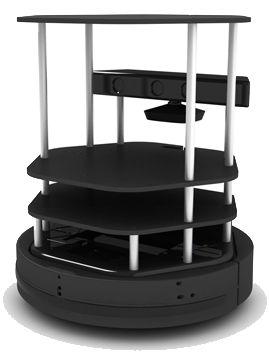
\includegraphics[scale=1.5]{figures/turtlebot.png}
  \caption{TurtleBot robot used in experiments.}
  \label{fig:turtlebot_pic}
\end{figure}


% !TEX root=../main.tex
\section{implementation}
\label{sec:implementation}


% !TEX root=../main.tex
\section{Results}
\label{sec:results}

We were pleased to be able to succesffully implement autonomous control of a
TurtleBot using an end-to-end visual control approach. The classical approach served as a meaningful learning experience and also a useful tool in collecting data to train the neural network approach, which was our end goal.

\begin{figure}[hbt]
  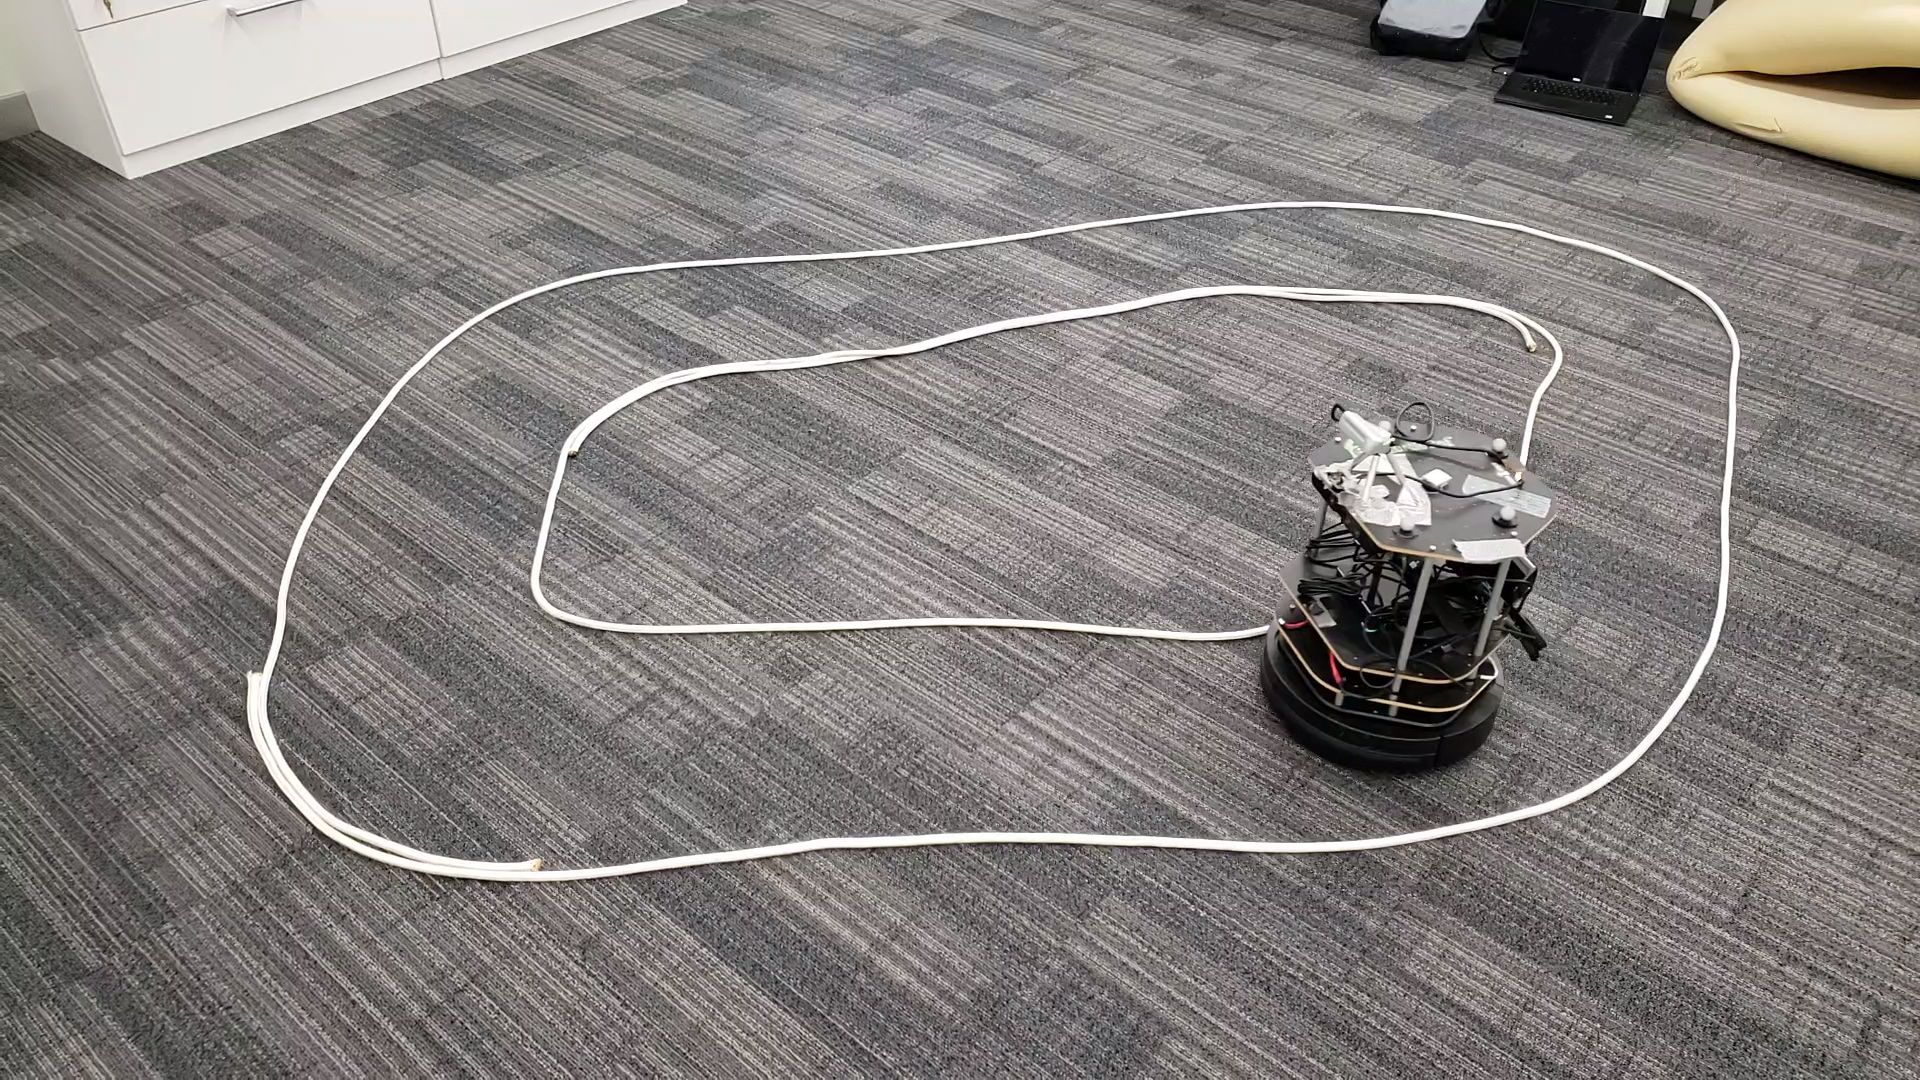
\includegraphics[width=\columnwidth]{figures/success_track}
  \caption{Snapshot of the TurtleBot successfully following a track using end-to-end deep learning-based control.}
  \label{fig:success_track}
\end{figure}

Some of the main advantages we saw of using the neural network control as opposed to the classical method was the ability to implicitly encode variability and robustness into the control simply by training on more data in varied environments. For example, the classical method, which depended heavily on proper segmentation, needed to be re-tuned for each ground surface and lighting condition, whereas the neural network was able to learn how to extract the proper features in multiple environments without the need to explicitly retune or revise the network.

It was also interesting to note the information the neural network was able to
learn. To visualize the salient features in a given image, we evaluated the
gradient of the output of the network with respect to the input image at the
given image. We then normalized these gradeints to turn them into a visible
grayscale image, equal in size to that of the input image. As seen in
Figures~\ref{fig:saliency1}~through~\ref{fig:saliency3}, the brightest pixels in
the gradient images correspond to the pixels that most contributed to the output
of the neural network. For the most part, these salient pixels correspond to the areas where the rope is seen in the input image. Note how the neural network learned to identify the rope specifically, not just white objects, as the light reflection in Figure~\ref{fig:saliency3} is filtered out and does not contribute much to the output. These glare spots were difficult for the classical method to handle, which conveys a clear advantage of the network-based control over the classical control.

\begin{figure}[hbt]
  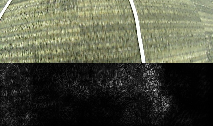
\includegraphics[width=\columnwidth]{figures/saliency1}
  \caption{Top: Original image; bottom: Class saliency for rope on carpet data. Shows the gradient is highest near where the rope appears in the original image (top)}
  \label{fig:saliency1}
\end{figure}

\begin{figure}[hbt]
  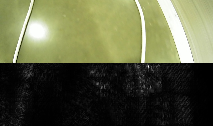
\includegraphics[width=\columnwidth]{figures/saliency2}
  \caption{Class saliency on reflective concrete flooring.}
  \label{fig:saliency2}
\end{figure}

\begin{figure}[hbt]
  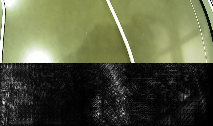
\includegraphics[width=\columnwidth]{figures/saliency3}
  \caption{Class saliency on reflecitve concrete floor with mulptiple glare spots. Show that the network learned to filter out bright contours that do not correspond with rope.}
  \label{fig:saliency3}
\end{figure}


% !TEX root=../main.tex
\section{Conclusion}
\label{sec:conclusion}




%%%%%%%%%%%%%%%%%%%%%%%%%%%%%%%%%%%%%%%%%%%%%%%%%%%%%%%%%%%%%%%%%%%%%%%
\bibliographystyle{IEEEtran}
\bibliography{library}

\end{document}
